\def\year{2019}\relax
%File: formatting-instruction.tex
\documentclass[letterpaper]{article} % DO NOT CHANGE THIS
\usepackage{aaai19}  % DO NOT CHANGE THIS
\usepackage{times}  % DO NOT CHANGE THIS
\usepackage{helvet} % DO NOT CHANGE THIS
\usepackage{courier}  % DO NOT CHANGE THIS
\usepackage[hyphens]{url}  % DO NOT CHANGE THIS
\usepackage{graphicx} % DO NOT CHANGE THIS
\urlstyle{rm} % DO NOT CHANGE THIS
\def\UrlFont{\rm}  % DO NOT CHANGE THIS
\usepackage{graphicx}  % DO NOT CHANGE THIS
\frenchspacing  % DO NOT CHANGE THIS
\setlength{\pdfpagewidth}{8.5in}  % DO NOT CHANGE THIS
\setlength{\pdfpageheight}{11in}  % DO NOT CHANGE THIS

\usepackage[utf8]{inputenc} % allow utf-8 input
\usepackage[UTF8]{ctex}
\usepackage{natbib}


%PDF Info Is REQUIRED.
% For /Author, add all authors within the parentheses, separated by commas. No accents or commands.
% For /Title, add Title in Mixed Case. No accents or commands. Retain the parentheses.
 \pdfinfo{
/Title (AAAI Press Formatting Instructions for Authors Using LaTeX -- A Guide)
/Author (AAAI Press Staff, Pater Patel Schneider, Sunil Issar, J. Scott Penberthy, George Ferguson, Hans Guesgen)
} %Leave this	
% /Title ()
% Put your actual complete title (no codes, scripts, shortcuts, or LaTeX commands) within the parentheses in mixed case
% Leave the space between \Title and the beginning parenthesis alone
% /Author ()
% Put your actual complete list of authors (no codes, scripts, shortcuts, or LaTeX commands) within the parentheses in mixed case. 
% Each author should be only by a comma. If the name contains accents, remove them. If there are any LaTeX commands, 
% remove them. 

% DISALLOWED PACKAGES
% \usepackage{authblk} -- This package is specifically forbidden
% \usepackage{balance} -- This package is specifically forbidden
% \usepackage{caption} -- This package is specifically forbidden
% \usepackage{color (if used in text)
% \usepackage{CJK} -- This package is specifically forbidden
% \usepackage{float} -- This package is specifically forbidden
% \usepackage{flushend} -- This package is specifically forbidden
% \usepackage{fontenc} -- This package is specifically forbidden
% \usepackage{fullpage} -- This package is specifically forbidden
% \usepackage{geometry} -- This package is specifically forbidden
% \usepackage{grffile} -- This package is specifically forbidden
% \usepackage{hyperref} -- This package is specifically forbidden
% \usepackage{navigator} -- This package is specifically forbidden
% (or any other package that embeds links such as navigator or hyperref)
% \indentfirst} -- This package is specifically forbidden
% \layout} -- This package is specifically forbidden
% \multicol} -- This package is specifically forbidden
% \nameref} -- This package is specifically forbidden
% \natbib} -- This package is specifically forbidden -- use the following workaround:
% \usepackage{savetrees} -- This package is specifically forbidden
% \usepackage{setspace} -- This package is specifically forbidden
% \usepackage{stfloats} -- This package is specifically forbidden
% \usepackage{tabu} -- This package is specifically forbidden
% \usepackage{titlesec} -- This package is specifically forbidden
% \usepackage{tocbibind} -- This package is specifically forbidden
% \usepackage{ulem} -- This package is specifically forbidden
% \usepackage{wrapfig} -- This package is specifically forbidden
% DISALLOWED COMMANDS
% \nocopyright -- Your paper will not be published if you use this command
% \addtolength -- This command may not be used
% \balance -- This command may not be used
% \baselinestretch -- Your paper will not be published if you use this command
% \clearpage -- No page breaks of any kind may be used for the final version of your paper
% \columnsep -- This command may not be used
% \newpage -- No page breaks of any kind may be used for the final version of your paper
% \pagebreak -- No page breaks of any kind may be used for the final version of your paperr
% \pagestyle -- This command may not be used
% \tiny -- This is not an acceptable font size.
% \vspace{- -- No negative value may be used in proximity of a caption, figure, table, section, subsection, subsubsection, or reference
% \vskip{- -- No negative value may be used to alter spacing above or below a caption, figure, table, section, subsection, subsubsection, or reference

\setcounter{secnumdepth}{0} %May be changed to 1 or 2 if section numbers are desired.

% The file aaai19.sty is the style file for AAAI Press 
% proceedings, working notes, and technical reports.
%
\setlength\titlebox{2.5in} % If your paper contains an overfull \vbox too high warning at the beginning of the document, use this
% command to correct it. You may not alter the value below 2.5 in
\title{基于条件生成对抗网络的配准多模态MRI合成}
%Your title must be in mixed case, not sentence case. 
% That means all verbs (including short verbs like be, is, using,and go), 
% nouns, adverbs, adjectives should be capitalized, including both words in hyphenated terms, while
% articles, conjunctions, and prepositions are lower case unless they
% directly follow a colon or long dash
\author{\Large \textbf{Yili Qu,Wanqi Su,Chufu Deng,Ying Wang,Yutong Lu,Nong Xiao,Zhiguang Chen}\\ % All authors must be in the same font size and format. Use \Large and \textbf to achieve this result when breaking a line
%\textsuperscript{\rm 1}Association for the Advancement of Artificial Intelligence\\ %If you have multiple authors and multiple affiliations
% use superscripts in text and roman font to identify them. For example, Sunil Issar,\textsuperscript{\rm 2} J. Scott Penberthy\textsuperscript{\rm 3} George Ferguson,\textsuperscript{\rm 4} Hans Guesgen\textsuperscript{\rm 5}. Note that the comma should be placed BEFORE the superscript for optimum readability
School of Data and Computer Science Sun Yet-Sen University\\	
quyli@mail2.sysu.edu.cn% email address must be in roman text type, not monospace or sans serif
}
 \begin{document}

\maketitle

\begin{abstract}
在基于大量数据驱动的医学影像智能处理任务中,医学影像数据的收集和采集是非常困难的,尤其是配准的多模态医学影像数据。合成的医学影像数据可以很好地缓解数据不足的问题。我们基于无监督的生成对抗网络模型实现了在已有单模态影像数据时可扩展出多模态影像数据并保留原模态的病灶信息,进一步实现了完全从随机噪声生成配准的多模态医学影像并可自由添加病灶信息。我们验证了合成的医学影像可以在医学影像智能处理任务与真实数据混合使用来提高模型的泛化能力。
\end{abstract}

\noindent 
核磁共振成像(MRI)是一种常见的医学影像,根据成像参数的不同可以有多种模态,例如T1、T2、T1c等。不同的模态对医生具有不同的参考价值,医生往往需要多个模态的影像互相对照才能做出准备的判断。在医学影像的智能处理任务的训练和学习中,我们往往也期望获得更多模态的影像,例如采用卷积神经网络(CNN)或生成对抗网络(GAN)进行的医学图像处理任务。

当同一个病人的同一个部位通过不同的成像技术得到不同的模态时,如果成像位置和视角一致的则被认为这些模态是配准的。相较于单模态数据,配准的多模态影像数据能提供更多的信息,可以支撑更多更复杂的应用场景,满足深度神经网络的训练数据的需求,有助于提供更加高效可靠的智能诊断服务。对于医生来说,获取不同模态的影像需要花费更长的时间并且需要患者的耐心配合,对于医学影像的智能处理任务的研究者来说,多模态的MRI数据集十分稀缺,收集难度非常大,尤其是罕见病,而配准的数据则更加稀少,这使得很多的训练任务无法实现。因此,通过应用图像合成技术扩展数据集,从已有的单模态图像转换为配准的多模态图像、从随机噪声生成配准的多模态医学影像,有着广泛的用途和深远的意义。

在GAN之前,一些研究使用图字典映射\cite{22burgos2015robust}、稀疏编码\cite{33huang2017simultaneous},\cite{34vemulapalli2015unsupervised},CNN\cite{36vannguyen2015crossdomain}等探索了医学影像的跨模态转换。此后许多研究使用GAN能产生更高质量的转换结果\cite{1zhao2018modular},\cite{5liang2018generative},\cite{6zhu2017unpaired},\cite{13choi2018stargan:}。得益于GAN的强大能力,目前,采用GAN实现跨模态医学影像转换成为主流\cite{2zhang2018translating},\cite{20nie2017medical},\cite{35osokin2017gans},\cite{36vannguyen2015crossdomain},\cite{40kamnitsas2017unsupervised}。一般的转换基于成对的数据,最近也有研究从不成对的跨域数据中学习\cite{2zhang2018translating}。最近的研究有将像素到像素的GAN应用于脑部MRI到CT图像的转换\cite{20nie2017medical},\cite{40kamnitsas2017unsupervised}、视网膜血管注释到图像的转换\cite{41costa2017towards}、基于CycleGAN\cite{6zhu2017unpaired}的心脏MRI到CT图像的相互转换与分割\cite{20nie2017medical}等。对于多模态的合成,[69]实现多输入多输出的MRI合成,但对输入的多模态数据要求配准。基于此,[45]改进实现存在缺失或未配准的多输入合成模型,能够从其输入的任何子集执行MRI图像合成,但限制了输出为单一模态,且模型不可扩展。[66]针对医学图像配准进行了深入研究。[4]应用GAN合成脑肿瘤图像实现数据增强和数据匿名化,但需要额外训练解剖结构分割网络,且要求数据集带有病灶分割标签,模型泛化能力弱。\cite{41costa2017towards}研究了基于变分自编码器(VAE)的思想实现血管注释图的随机生成,进而合成彩色视网膜图像。在当前的这些医学影像合成的研究中,大多仅探索了两个不同模态之间的转换\cite{2zhang2018translating},\cite{20nie2017medical},\cite{22burgos2015robust},\cite{34vemulapalli2015unsupervised},\cite{35osokin2017gans},\cite{36vannguyen2015crossdomain},\cite{40kamnitsas2017unsupervised},对多模态的研究还很稀少[69,4],而在医学影像处理领域之外,多域转换的发展最近已经有了进展\cite{1zhao2018modular},\cite{5liang2018generative},\cite{13choi2018stargan:},\cite{27isola2017image-to-image}。

目前针对医学影像合成的研究存在模态数量难以扩展、需要配准训练数据、依赖于复杂的大型网络、无法添加或保留病灶、需要从真实数据扩展而无法从随机矩阵开始生成、需要额外的训练数据等各项问题,且大多数研究对合成数据的评价依赖于经验医师的人工视觉效果评估,没有进行客观的量化检验。因此,我们设计了一种基于生成对抗网络的多模态配准图像生成的方法,采用无监督学习方法,训练数据无需配准,可以接收一个符合我们设计规范的随机输入,进而生成一组有标签的多模态配准图像。具体来说,我们的贡献体现在以下三个方面:
\begin{itemize}
\item \textbf{结构特征图的提取与随机生成}
我们针对医学影像提出了一种解剖结构特征的提取方法,无需额外的解剖结构分割标签无需额外提取训练,可直接从任意模态的真实影像提取得到结构特征,用以辅助生成对抗网络学习生成更合理的合成影像。我们训练了一个结构特征图生成器实现了从多维正态分布生成结构特征图。我们的提取方法可以直接获取真实影像的解剖结构特征,在提升合成影像质量同时不带来额外参数、计算开销小,而随机生成方法可以无限地生成丰富多样的结构特征图。
\item \textbf{带标签多模态配准影像的合成}
我们使用随机生成的结构特征图,融合随机选择的病灶信息标签,通过生成器合成配准的多模态MRI。在训练时我们无需配准的数据,除病灶信息标签外无需额外的数据标签,而合成的数据是配准的,且输入的随机选择病灶信息标签即为合成数据的病灶信息标签。我们的方法能够便捷快速地构建带标签的配准多模态MRI数据集。
\item \textbf{病灶有效性和数据可用性的客观验证方法}
我们通过训练好的真实影像的病灶分割网络,对合成数据进行病灶分割测试,验证合成数据的病灶信息是否符合对应的病灶信息标签。此外,我们还使用不同比重的合成数据和真实数据构建的数据集来训练病灶分割网络,验证了合成数据可以在医学影像智能处理任务与真实数据混合使用来提高模型的泛化能力。对比传统合成影像质量的主观评价方法,我们的方法能客观真实地验证合成数据中病灶信息的有效性以及合成数据的可用性。
\end{itemize}

\section{方法}
\subsection{整体架构}
\begin{figure}
	\centering
	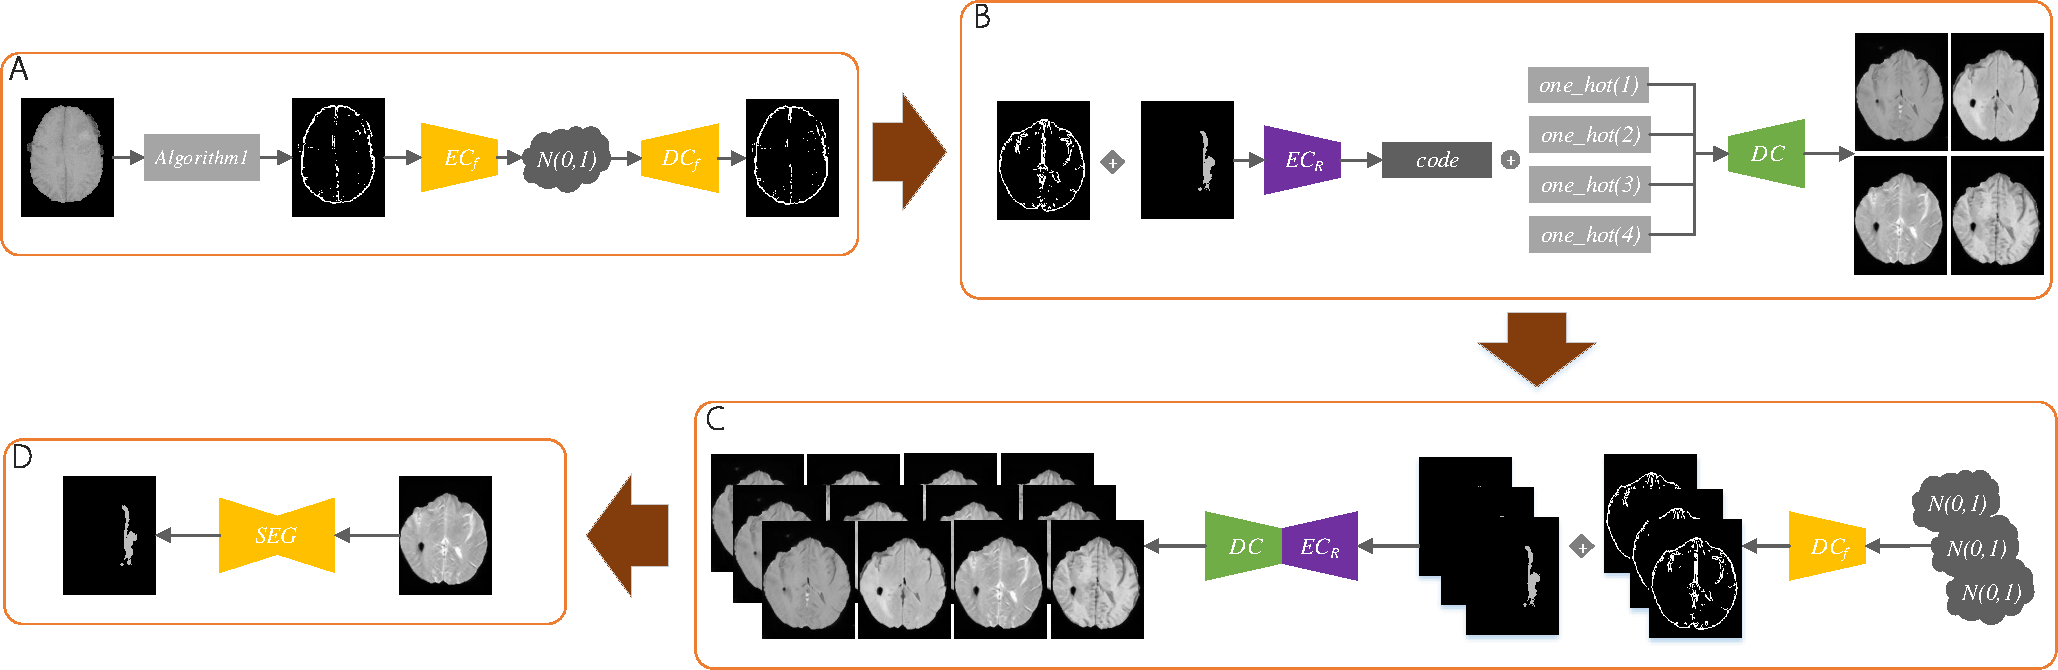
\includegraphics[width=0.98\linewidth]{figures/architecture}
	\caption{整体架构图.}
	\label{architecture}
\end{figure}
如图\ref{architecture}所示,我们的方法包括结构特征图提取和生成、多模态MRI生成、构建合成数据集、合成数据分割检测四个主要阶段。

结构特征图提取和生成阶段我们将获得一个结构特征图生成器,能从随机的正态分布矩阵生成结构特征图。该阶段我们训练的模型模包括一个结构特征图编码器、一个结构特征图解码器和一个结构特征图鉴别器。

多模态MRI生成阶段我们产出一个条件生成器,其以结构特征图为输入,能根据不同的独热条件向量生成不同模态的MRI,并且可在结构特征图上添加病灶标签使得生成的MRI具有对应的病灶信息。该阶段我们训练的模型模块包括一个结构特征与病灶标签融合图编码器、一个病灶标签解码器、一个MRI编码器、一个MRI解码器、一个MRI鉴别器和一个MRI编码鉴别器。

在构建合成数据集阶段,我们使用前两个阶段产出的模型先从随机正态分布矩阵生成足量的结构特征图再随机添加病灶标签,最后生成配准的多模态MRI,构建出一个合成数据集。

在合成数据分割检测阶段,我们根据真实的数据为每个模态的MRI单独训练一个病灶分割网络,并在真实数据集中进行分割能力测试。然后我们使用训练好的分割器对合成数据集中的MRI进行分割,将分割结果与添加的病灶标签比对评估,以此检验生成的MRI中包含了我们预期的病灶信息。此外,我们使用由不同比重的合成数据和真实数据构建的数据集来对病灶信息检测阶段中的病灶分割网络进行训练,训练充分后再在真实测试数据集上进行分割能力测试,对比各项测试结果,以验证合成数据在模型训练中的可用性。该阶段我们训练的模型包括每个模态的MRI的基于不同数据比重的病灶分割器。

\subsection{结构特征图提取方法}
结构特征图指医学影像中提供解剖结构信息或血管分布信息的图像,如常用的分割标签图和血管注释图,这些结构特征图通常无法使用生成对抗网络直接从随机噪声生成获取,因为这样的网络很难训练,且生成的结构特征图效果不好、不具备真实的结构信息。而现有的手段一般是训练一个解剖结构分割网络,从模态图得到分割标签,但这需要大量的数据分割标签和额外的训练过程,在使用时仍然需要真实的模态图作为输入来得到生成的解剖分割标签,这大大降低了生成数据的多样性。对此,我们设计了从模态图直接提取结构特征图的方法,并在这种提取方法的基础上,进一步设计从符合规范的随机噪声生成结构特征图的方法,提高生成数据的多样性。

目前,利用生成对抗网络,可以实现从随机噪声生成具有细节纹理的医学影像,但这样的生成网络一是难训练,二是生成的影像不具有符合事实的解剖结构,因此生成的影像不够保真,所以通常需要添加结构特征辅助训练以使结果更逼真,而现有的手段一般是添加解剖结构分割图,这要求数据集有对应的分割标签或需要额外训练分割网络。为了解决这个问题,本研究将基于传统数字图像处理方法设计一个结构特征图提取方法,能够直接从真实医学影像提取结构信息。Roberts算子、Prewitt算子、Sobel算子等传统的边缘检测方法具有运算快、无需训练、无需额外数据等优点。本研究将在这类传统的边缘检测算子的基础上探索新的简单高效的医学影像结构特征提取方法。

对一张真实图像n,用Sobel算子提取得到结构图,对结构图进行一系列操作得到最小值图和最大值图,两者加和得到结构特征图,具体算法见如下伪码:
\begin{quote}
	\begin{scriptsize}\begin{verbatim}
	算法1 结构特征图提取
	1:输入一张真实图像n,beta为元素阈值
	2:f1 = reduce_min(sobel(n))
	3:f2 = reduce_max(sobel(n))
	4:f1 = mean(f1) - f1
	5:f2 = f2 - mean(f2)
	6:f1 = ones * (f1 > beta)
	7:f2 = ones * (f2 > beta)
	8:f = f1 + f2
	9:f = ones * (f > 0.)
	\end{verbatim}\end{scriptsize}
\end{quote}

\subsection{随机结构特征图的生成训练}
本研究目标为合成大量的影像构建数据集,所以合成的影像必须保持多样性。从随机噪声生成的图像具有多样性,因此需要解决从随机噪声生成结构特征图这一问题。本研究结合变分自编码器与生成对抗网络,将从真实影像提取得到的结构特征图编码为一个潜在特征,通过约束潜在特征服从多维正态分布,实现从多维正态分布随机采样生成结构特征图,对真实的提取结构特征图与随机生成的结构特征图进行对抗学习,使生成的结构特征图越来越逼真。
\begin{quote}
	\begin{scriptsize}\begin{verbatim}
		算法2 掩模提取
		1:输入一张真实图像n,p为扩充元素值
		2:mask = 1.0 - ones * (n > 0.)
		3:shape = get_shape(n)
		4:mask = resize(mask, size=[shape[1] + p, shape[2] + p])
		5:mask = resize_with_crop_or_pad(mask, shape[1], shape[2])
		\end{verbatim}\end{scriptsize}
\end{quote}
这一部分独立训练,训练完成后,生成的随机结构特征图用于进一步生成一组有分割标签的配准的多模态数据。如图所示,从标准正态分布解码得到随机结构特征图的具体处理过程如下:
\begin{itemize}
	\item 每次随机选择一个模态,从这个模态中获取一张图n,用结构特征提取方法得到结构特征图F,用掩模提取方法得到对应掩模Mask;
	\item 用编码器$Encoder_F$对结构特征图F进行编码获得$Code_(F,mean)$及$Code_(F,logvar)$,从正态分布$N(0,1^2)$的获取随机噪声$Code_e$,由三个编码求得$Code_F=Code_(F,mean)+exp(0.5*Code_(F,logvar) )*Code_e$;
	\item 用解码器$Decoder_F$对$Code_F$解码得到重建的结构特征图$F_r$;
	\item 用解码器$Encoder_Mask$ 、$Decoder_Mask$从$F$提取得到掩模$Mask_r$;
	\item 随机生成符合正态分布$N(0,1^2)$的矩阵$Code_(F,RM)$;
	\item 用解码器$Decoder_F$对$Code_(F,RM)$解码得到生成的随机结构特征图$F_RM$;
	\item 用解码器$Encoder_Mask$ 、$Decoder_Mask$对$F_RM$提取得到掩模$Mask_RM$;
	\item 结构特征图鉴别器$Discriminator_F$分别对$F$和$F_RM$进行鉴别,将前者鉴别为真,后者鉴别为假;
	\item 结构特征鉴别器$FeatureDiscriminator_F$分别对$Code_F$和$Code_(F,RM)$进行鉴别,将前者鉴别为假,后者鉴别为真。
\end{itemize}

在训练过程中,我们希望随机正态分布矩阵解码出结构特征图更逼真,所以通过鉴别器$Discriminator_F$对原图提取的结构特征及掩模与随机正态分布矩阵解码的结构特征及掩模进行对抗学习,此外,还添加了编码特征的GAN,通过结构特征鉴别器$FeatureDiscriminator_F$对真实结构特征图编码结果$Code_F$与服从标准正态分布的矩阵$Code_(F,RM)$进行对抗学习,以此使得编码器$Encoder_F$能够将结构特征图F编码为服从标准正态分布的结果。
损失函数如下:

使得结构特征图编码服从正态分布的对抗性损失

$
loss_(FeatureDiscriminator,1)=‖FeatureDiscriminator_F (Code_(F,RM) )-1‖_2^2×ω_1  +‖FeatureDiscriminator_F (Code_F )-0‖_2^2×ω_2
loss_(Generator,1)=‖FeatureDiscriminator_F (Code_F )-1‖_2^2×ω_3  $

其中,$ω_i$为各项损失的权重,0和1表示真实与否。

使得结构特征图中间编码结果服从正态分布的自监督损失

$loss_(Supervision,1)=‖〖mean(Code〗_(F,mean))-0‖_2^2×ω_4+ ‖mean(exp(0.5*Code_(F,logvar) ))-1‖_2^2×ω_5$

使得随机正态分布矩阵解码出结构特征图更逼真的对抗性损失

$loss_(Discriminator,1)=‖Discriminator_F (F)-1‖_2^2×ω_6+‖Discriminator_F (F_RM )-0‖_2^2×ω_7
loss_(Generator,2)=‖Discriminator_F (F_RM )-1‖_2^2×ω_8$

结构特征图和掩模两次重建融合后与原始结构特征图和掩模的两两自监督一致性损失

$loss_(Supervision,2)=‖F-F_r ‖_2^2×ω_9+‖F_r*Mask‖_2^2×ω_11$

从$f$生成对应$mask$的MASK生成器损失

$loss_mask=‖Mask〖-Mask〗_r ‖_2^2×ω_10+‖F〖*Mask〗_r ‖_2^2×ω_12+‖F_r 〖*Mask〗_r ‖_2^2×ω_13+‖F_RM*Mask_RM ‖_2^2×ω_14$

\subsection{结构图与肿瘤标签的融合方法}
通过(5)我们可以得到从标准正态分布随机生成的结构特征图$F_RM$,然后我们随机选择分割标签图L,将包含5个类别的分割标签图转为独热矩阵,得到一个通道数与类别数量一样的多维标签矩阵,每个通道中仅有部分像素有效,其余部分为填充的0,这些非0像素区域与分割标签图中的各个分割区域是配准的。最后,我们将这个被分割后的多维标签矩阵与结构特征图一起在通道维度进行堆叠,得到一个融合了两个输入源的输入矩阵作为最终输入。

\subsection{多模态MRI生成训练}
目前,多模态数据生成的方案有:①基于解剖结构分割标签生成多模态影像,这种方法依赖于数据集中的解剖结构分割标签,生成的多模态影像数量是有限的,生成影像不具备多样性;②从随机噪声生成多模态影像,这种方法通常很难训练得到合理的模态图,即使能生成符合语义特征的影像,生成影像中也不具备符合事实的解剖结构。针对以上问题,本项目将基于前项生成随机结构特征图的研究,进一步研究从随机结构特征图生成多模态数据的方法,使多模态数据的生成训练更容易,生成的多模态数据保持多样性、更加合理和逼真。

结构特征图包含了目标部位主要的解剖结构信息,从结构特征图生成模态图比直接从随机噪声生成模态图更易训练,生成的模态图更加合理和逼真。本研究使用一个单独的编码器对结构特征图进行编码,通过鉴别器损失使得编码得到的语义特征图逼近模态图编码后的语义特征图所在潜在空间,然后使用模态转换方法中的模态解码器对结构特征图编码得到的语义特征图进行解码,得到各个模态的模态图,再通过一系列循环重建约束和互转一致性约束保证生成的多模态影像互相配准。此外,本研究将输入的随机病灶信息标签与生成的多模态影像再编码后重建得到的病灶信息标签进行对抗学习,确保生成的多模态影像根据输入病灶标签生成了对应的病灶内容。

训练过程如图所示:

在以上图像生成训练过程中,由于结构特征图$F_1$是从随机图像$n$中提取的,提取出的结构特征有可能包含肿瘤结构信息,会干扰与随机标签L中的肿瘤信息,影响融合后生成的图像,所以$F_1$需要在与随机标签L融合前消除肿瘤信息,得到无肿瘤信息的结构特征图$F$,使生成图像的肿瘤信息只来源于标签$L$。

在训练过程中我们通过设计损失函数作为模型的学习准则,约束模型的优化方向。

使得随机正态分布矩阵解码出结构特征图更逼真的对抗性损失

$loss_(Discriminator,Adversarial )=Σ_(i=0)^(C-1) 〖(‖Discriminator_F (x_i )[0]-1‖〗_2^2×ω_6+‖Discriminator_F (x_(g,i) )[0]-0‖_2^2×ω_7)
loss_(Generator,Adversarial )=Σ_(i=0)^(C-1) ‖Discriminator_F (x_(g,i) )[0]-1‖_2^2×ω_8$

模态类别指导损失

$loss_(Discriminator,class )=Σ_(i=0)^(C-1) (‖Discriminator_F (x_i )[1]-i‖_2^2×ω_6+‖Discriminator_F (x_(g,i) )[1]-i‖_2^2×ω_(7))
loss_(Generator,class)==Σ_(i=0)^(C-1) ‖Discriminator_F (x_(g,i) )[1]-i‖_2^2×ω_8$

输入的结构特征图的重建自监督损失

$loss_(supervision,3)=〖Σ_(i=0)^(C-1) ‖F-F_(x,i,g) ‖〗_2^2×ω_20$

与输入的结构特征图融合后输入的肿瘤分割标签图的重建自监督损失

$loss_(supervision,4)=‖L-L_r ‖_2^2×ω_20+Σ_(i=0)^(C-1) ‖L-L_(x,i,g) ‖_2^2×ω_20$

生成的模态图进行转换得到的转换图与生成图的自监督损失

$loss_(supervision,6)=Σ_(j=0,j≠i)^(C-1) Σ_(i=0)^(C-1) ‖x_(g,i)-x_(g,i,j,t) ‖_2^2×ω_20$

通过解码器生成X模态与Y模态图的编码与X模态与Y模态图经过编码器得到的编码的自监督语义一致性损失

$loss_(Supervision,9)=〖Σ_(i=0)^(C-1) ‖Code_RM-Code_(x,i,g) ‖〗_2^2×ω_4+ Σ_(j=0,j≠i)^(C-1) Σ_(i=0)^(C-1) ‖Code_(x,i,g)-Code_(x,j,g) ‖_2^2×ω_4$

上述公式中,$ω_i$为各项损失的权重。

\subsection{辅助的模态重建和模态转换训练}
现有的医学影像模态转换方案大多关注MRI与CT、MRI两个子模态、CT低剂量图与高剂量图之间的两模态互转,很少有针对已有单模态数据转换生成多模态数据的方案,因为这些两模态方案通常不可扩展或扩展代价很大,且要求数据集配准。为此,本项目将研究从已有的单模态数据转换生成多模态数据的方法,实现模态扩展同时生成的配准的多模态数据。

为了能够实现配准的多模态影像生成,首先需要实现多模态的互转。本研究基于生成对抗网络,将生成器模块化为编码器和解码器,每个模态对应一个编码器和一个解码器。对每个模态进行模态转换和模态重建。模态转换时,编码器将模态图编码得到语义特征图,通过各个其他模态的解码器解码出全部的模态转换图。然后对所有转换图用对应模态编码器进行再编码得到的语义特征图,最后通过原始模态的解码器全部解码得到循环重建的原始模态图。模态重建时,编码器将模态图编码得到语义特征图,然后通过模态解码器解码得到重建模态图。最后用一系列循环重建约束和互转一致性约束保证转换的多模态影像互相配准。通过上述方法,可无监督地实现单模态转换生成多模态配准数据。

如图所示,模态数量为$C$时,对任意一个模态m,我们一共进行$C-1$次模态转换、一次模态重建。模态转换时,编码器将$m$模态的MRI编码得到语义特征图$code_m$ ,然后我们将其与不同的条件向量连接,通过解码器解码出全部的模态。当解码还原到$m$模态本身时,即是该模态的模态重建。对所有通过模态转换得到的转换图,我们全部采用编码器进行再编码,将全部再编码得到的语义特征图均与$m$模态的条件向量进行连接,最后再用解码器全部解码得到循环重建的$m$模态的MRI。注意,模态重建得到的重建图无需再编码和循环重建。模态重建的循环重建都是自监督训练。真实模态图与模态转换的道德转换图分别作为鉴别器的正样本和负样本,通过鉴别器提供的对抗性损失实现无监督训练。

在上述过程中,原始输入模态$m$对应的病灶标签$label_m$作为病灶还原训练的监督标签。具体来说,上述过程中由原始输入的$m$模态的MRI得到的一个经过编码得到语义特征图和$C-1$个经过再编码得到的语义特征图,全部通过病灶解码器生成病灶标签图,$label_m$作为监督标签。

训练采用的学习率、优化方法等超参数设置均可根据任务实际情况自由配置。

我们的鉴别器模块独立更新,其损失为:

$〖loss〗_Discriminator=Σ_(j=0,j≠i)^(C-1) Σ_(i=0)^(C-1) (‖Discriminator(x_(t,i,j) )[0]-0‖_2^2×ω_(3,i,j))+Σ_(j=0,j≠i)^(C-1) Σ_(i=0)^(C-1) (‖Discriminator(x_(t,i,j) )[1]-i‖_2^2×ω_(4,i,j))$

其中$x_i$指真实的编号为i的模态的MRI,$x_(t,i,j)$指由编号为$j$的模态转换生成的编号为$i$的模态的MRI,$ω$为损失项的权重,0与1表示真实与否,$i$表示模态类别。

我们其他模块通过一个优化器更新训练,损失项包括鉴别器提供的对抗性损失、模态重建自监督损失、模态循环重建自监督损失、模态循环重建一致性损失、语义一致性损失、病灶监督损失、病灶一致性损失。具体来说:

对抗性损失

$loss_(Adversarial )=Σ_(j=0,j≠i)^(C-1) Σ_(i=0)^(C-1) (‖Discriminator(x_(t,i,j) )[0]-1‖_2^2×ω_(3,i,j))+Σ_(j=0,j≠i)^(C-1) Σ_(i=0)^(C-1) (‖Discriminator(x_(t,i,j) )[1]-i‖_2^2×ω_(4,i,j))$

模态重建自监督损失

$loss_rebuild=Σ_(i=0)^(C-1) ‖x_i-x_(r,i) ‖_2^2×ω_(5,i)$

其中$x_(r,i)$表示编号为$i$的模态重建得到的$i$模态的MRI。

模态循环重建自监督损失

$loss_(cycle,rebuild)=Σ_(j=0,j≠i)^(C-1) Σ_(i=0)^(C-1) ‖x_i-x_(cr,i,j) ‖_2^2×ω_(6,i,j)$

其中$x_(cr,i,j)$表示编号为i的模态转换到编号为$j$的模态再转换回的$i$模态的MRI。
模态循环重建一致性损失

$loss_(cycle,consistency)=Σ_(k=0,k≠j,k≠i)^(C-1) Σ_(j=0,j≠i)^(C-1) Σ_(i=0)^(C-1) ‖x_(cr,i,j)-x_(cr,i,k) ‖_2^2×ω_(7,i,j,k)$

其中$i、j、k$表不同的模态。

语义一致性损失

$loss_(code,consistency)=Σ_(j=0,j≠i)^(C-1) Σ_(i=0)^(C-1) ‖〖code〗_i-〖code〗_(t,i,j) ‖_2^2×ω_(8,i,j)+Σ_(k=0,k≠j,k≠i)^(C-1) Σ_(j=0,j≠i)^(C-1) Σ_(i=0)^(C-1) ‖〖code〗_(t,i,j)-〖code〗_(t,i,k) ‖_2^2×ω_(9,i,j,k)$

其中,$〖code〗_i$表示编号为i的模态的MRI经过编码器编码后得到的语义特征图,$〖code〗_(t,i,j)$表示由编号为$j$的模态转换生成的编号为$i$的模态的MRI经过编码器编码后得到的语义特征图。

病灶监督损失

$loss_label=Σ_(i=0)^(C-1) ‖〖label〗_i-〖label〗_(g,i) ‖_2^2×ω_(10,i)$

其中$〖label〗_i$表示编号为i的模态的MRI的真实病灶标签,$〖label〗_(g,i)$表示编号为i的模态的MRI经过编码器编码后再经过病灶解码器解码生成的病灶标签,$〖label〗_(t,i,j)$表示由编号为i的模态转换生成的编号为$j$的模态的MRI经过编码器编码后再经过病灶解码器解码生成的病灶标签。

\subsection{构建合成数据集}
为了能够实现配准的多模态影像生成,首先需要实现多模态的互转。本研究基于生成对抗网络,将生成器模块化为编码器和解码器,每个模态对应一个编码器和一个解码器。对每个模态进行模态转换和模态重建。模态转换时,编码器将模态图编码得到语义特征图,通过各个其他模态的解码器解码出全部的模态转换图。然后对所有转换图用对应模态编码器进行再编码得到的语义特征图,最后通过原始模态的解码器全部解码得到循环重建的原始模态图。模态重建时,编码器将模态图编码得到语义特征图,然后通过模态解码器解码得到重建模态图。最后用一系列循环重建约束和互转一致性约束保证转换的多模态影像互相配准。通过上述方法,可无监督地实现单模态转换生成多模态配准数据。

我们通过训练好的结构特征图解码器即可从随机生成的正太分布矩阵生成无限的结构特征图,然后,我们再将随机生成的结构特征图和随机选择的病灶信息标签融合,通过多模态生成模型即可生成配准的多模态影像,选取的病灶信息标签就是生成的多模态影像的病灶标签。由此,我们可以从随机矩阵构建带有病灶标签的多模态配准影像数据集。

\subsection{病灶分割网络训练}
在医学影像中,病灶信息是医生在诊断时最关注的信息,现有的医学影像处理任务最终也是为诊断服务的,所以带病灶信息标签的数据集的价值很高,而目前对于合成有病灶信息的影像数据的研究还很少。对此,本项目将研究添加病灶信息标签合成的多模态数据的方法,使病灶信息标签与前项研究的结构特征图融合后,进一步合成能够保留病灶信息的多模态数据。

为了验证合成数据病灶信息来源于随机输入的病灶标签且与其保持一致,本研究根据真实的数据为每个模态单独训练一个病灶分割网络,并在真实数据集中进行分割能力测试。然后使用训练好的分割器对合成数据集中的影像进行分割,将分割结果与输入的病灶标签比对评估,以此检验合成的影像中包含了预期的病灶信息。

现有的研究对合成数据的评估是不充分的,大多研究只通过均方误差(MSE)、峰值信噪比(PSNR)、结构相似性(SSIM)这三个指标评价合成数据与原数据的相似度,以此对合成数据的质量进行定量评估,部分研究还会请经验医师对合成数据的视觉效果进行定性评估,这些评估方法都只对合成数据进行了质量评估,没有真正的评估这些合成数据是否可用,合成数据包含的病灶信息与其病灶标签是否对应。针对以上问题,本项目将设计一种合成数据有效性评估的方法,以及一种病灶信息检测验证方法,客观的评价合成数据是否可用、病灶标签是否有效。

本研究使用由不同比重的合成数据和真实数据构建的数据集来对病灶信息检测中的病灶分割网络进行训练,训练充分后再在真实测试数据集上进行分割能力测试,对比各项测试结果,以验证合成数据在模型训练中的可用性。

\section{实验}
\subsection{数据集与数据预处理}
\subsection{训练设置}
\subsection{病灶检测实验}
\subsection{合成数据可用性验证实验}

\section{结果}
\subsection{实验量化结果}
\subsection{实验可视化结果}

\section{结论与未来工作}

\section{ Acknowledgments}
在基于大量数据驱动的医学影像智能处理任务中,医学影像数据的收集和采集是非常困难的,尤其是配准的多模态医学影像数据。合成的医学影像数据可以很好地缓解数据不足的问题。生成对抗网络在计算机视觉任务中取得了广泛和稳定的优秀表现。我们基于当前表现优秀的生成对抗网络模型,通过无监督的训练,实现在已有单模态数据时可扩展出多模态影像数据并保留原模态的病灶信息,进一步实现完全从随机噪声生成配准的多模态医学影像并可自由添加病灶信息。合成的医学影像可以用于医学影像智能处理任务的预训练或者补充训练来提高模型的泛化能力。

当前,医学影像智能处理依赖大量的数据,而由于医学影像的采集的困难,现有的公开数据集数据量较少,配准数据和病灶标签稀缺。因此,本项目的研究目标是通过现有数据构建合成带标签的多模态配准医学影像数据集,用作医学影像智能处理任务的预训练或者补充训练。具体研究目标包括:
\begin{itemize}
	\item 设计结构特征图提取方法,从医学影像直接提取解剖结构信息,给影像合成提供解剖结构信息,辅助训练使合成影像更逼真;
	\item 设计随机结构特征图生成方法,实现从多维正态分布采样生成结构特征图,使结构特征图能便捷地大量生成并使最后合成的影像保持多样性;
	\item 设计模态转换方法,实现多模态之间的互转,使单模态数据可转换生成多模态影像数据并保留原模态的病灶信息;
	\item 设计基于结构特征图生成多模态图方法,从真实影像提取的结构特征图及随机选择的标签生成配准的多模态影像;
	\item 设计构建带标签的多模态配准数据集方法,重组训练好的部件,实现从多维正态分布随机生成结构特征图,结合随机选择的标签生成多模态配准的影像数据;
	\item 设计合成数据病灶信息检测方法,检验合成的数据中是否包含预期的病灶信息,以此保证病灶信息的有效性;
	\item 设计合成数据有效性测试方法,将合成数据用于原数据集的任务处理,以验证合成数据在模型训练中的可用性。
\end{itemize}	
通过以上研究,本项目将实现从单模态数据扩展为多模态数据,从随机输入生成多模态配准影像数据,并通过若干测试验证方案的有效性。

\bibliographystyle{plain}

\bibliography{refer}

\end{document}
